\ifSTANDALONE
    \section{Schrittmotor} \label{sec:stepper}
\fi
\ifEMBED
    \subsection{Schrittmotor} \label{sec:stepper}
\fi
\ifEMBED
    % Dieses Kapitel ist eine Zusammenarbeit der Gruppen \BLDCTeams. 
    \BLDCcollab
\fi
    Schrittmotoren oder auch Stepper genannt, sind Synchronmotoren, bei 
    welchen der Rotor um einen bestimmten Winkel gedreht werden kann. So ist 
    die Rotorposition ohne zusätzliche Sensoren bekannt. Dabei ist zu 
    beachten, dass der Motor keine Schritte verliert, was bei Überlast 
    geschehen kann. Da die meisten Schrittmotorensysteme Open- Loop Systeme 
    sind, entsteht eine dauernde Positionsabweichung bei einem Schrittverlust. 
    Grundsätzlich wird zwischen zwei Schrittmotortypen unterschieden: 
    \begin{itemize}
       	\item Permanentmagnetmotor
       	\item Reluktanzmotor
    \end{itemize} 
    Der Permanentmagnetmotor besitzt als Rotor einen Permanentmagneten. Beim 
    Reluktanzmotor besteht der Rotor aus einem gezahnten Weicheisenkern. 
    Permanentmagnetmotoren erreichen eine kleinere Schrittfrequenz, besitzen 
    jedoch ein grösseres Drehmoment als Reluktanzmotoren. Die Kombination 
    aus Reluktanzmotor und Permanentmagnetmotor ist ein Hybridmotor. Ein 
    Hybridmotor verbindet die Vorteile von Reluktanz- und Permanentmotor. 

\ifSTANDALONE
    \subsection{Schritte} \label{sec:steps}
\fi
\ifEMBED
    \subsubsection{Schritte} \label{sec:steps}
\fi
    Der Vollschrittbetrieb kann ein- oder auch zweiphasig gesteuert 
    werden. Beim einphasigen Vollschrittbetrieb sind immer zwei gegenüber 
    liegende Pole aktiv. Beim zweiphasigen Vollschrittbetrieb werden jeweils 
    zwei nebeneinander liegende Pole aktiv. Im Halbschrittbetrieb werden die 
    beiden Vollschrittbetriebsarten kombiniert. So kann der Schrittwinkel 
    halbiert werden. Zusätzlich kann der Schrittmotor mit Mikroschritten 
    betrieben werden. Dabei folgt der Strom der sinusförmigen 
    Referenzspannung. (Vgl. Seite \pageref{stromgesteuert}) 
    \begin{figure}[h!]
    	\centering
    	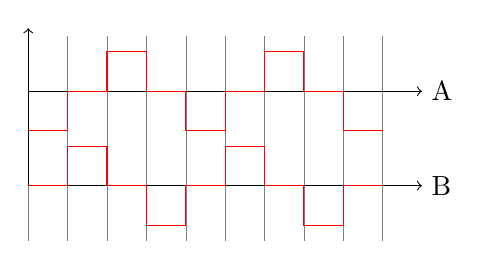
\begin{tikzpicture}
        % Hilfslinien
        \foreach \i in {0, 0.5, ..., 4.5}
        {
            \draw[ultra thin, gray] (\i, 1.9) -- (\i, -0.7);
        }
        % Achsen
    	\draw[->]	(0, 0) -- (0, 2);
    	\draw[->]	(0, 1.2) -- (5, 1.2) node[right]{A};
    	\draw[->]	(0, 0) -- (5, 0) node[right]{B};
        % Kurven
        \draw[red] 
            (0     ,0.7) --
            (0.5   ,0.7) --
            (0.5   ,1.2) --
            (1     ,1.2) --
            (1     ,1.7) --
            (1.5   ,1.7) --
            (1.5   ,1.2) --
            (2     ,1.2) --
            (2     ,0.7) --
            (2.5   ,0.7) --
            (2.5   ,1.2) --
            (3     ,1.2) --
            (3     ,1.7) --
            (3.5   ,1.7) --
            (3.5   ,1.2) --
            (4     ,1.2) --
            (4     ,0.7) --
            (4.5   ,0.7);
        \draw[red] 
            (0      ,0) --
            (0.5    ,0) --
            (0.5    ,0.5) --
            (1      ,0.5) --
            (1      ,0) --
            (1.5    ,0) --
            (1.5    ,-0.5) --
            (2      ,-0.5) --
            (2      ,0) --
            (2.5    ,0) --
            (2.5    ,0.5) --
            (3      ,0.5) --
            (3      ,0) --
            (3.5    ,0) --
            (3.5    ,-0.5) --
            (4      ,-0.5) --
            (4      ,0) --
            (4.5    ,0) ;
    	\end{tikzpicture}
    	\caption{Vollschritt}
    	\label{fig:vollschritt}
    \end{figure}
    \begin{figure}[h!]
     	\centering
     	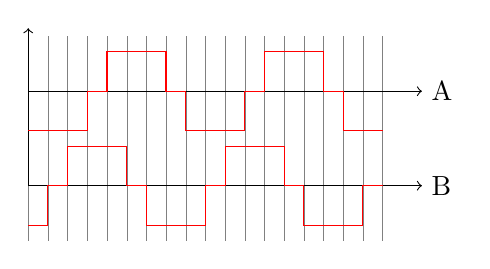
\begin{tikzpicture}
        % Hilfslinien
        \foreach \i in {0, 0.25, ..., 4.5}
        {
            \draw[ultra thin, gray] (\i, 1.9) -- (\i, -0.7);
        }
        % Achsen
    	\draw[->]	(0, 0) -- (0, 2);
    	\draw[->]	(0, 1.2) -- (5, 1.2) node[right]{A};
    	\draw[->]	(0, 0) -- (5, 0) node[right]{B};
        % Kurven
        \draw[red] 
            (0     ,0.7) --
            (0.75   ,0.7) --
            (0.75   ,1.2) --
            (1     ,1.2) --
            (1     ,1.7) --
            (1.75   ,1.7) --
            (1.75   ,1.2) --
            (2     ,1.2) --
            (2     ,0.7) --
            (2.75   ,0.7) --
            (2.75   ,1.2) --
            (3     ,1.2) --
            (3     ,1.7) --
            (3.75   ,1.7) --
            (3.75   ,1.2) --
            (4     ,1.2) --
            (4     ,0.7) --
            (4.5   ,0.7);
        \draw[red] 
            (0      ,-0.5) --
            (0.25   ,-0.5) --
            (0.25   ,0) --
            (0.5    ,0) --
            (0.5    ,0.5) --
            (1.25   ,0.5) --
            (1.25   ,0) --
            (1.5    ,0) --
            (1.5    ,-0.5) --
            (2.25   ,-0.5) --
            (2.25   ,0) --
            (2.5    ,0) --
            (2.5    ,0.5) --
            (3.25   ,0.5) --
            (3.25   ,0) --
            (3.5    ,0) --
            (3.5    ,-0.5) --
            (4.25   ,-0.5) --
            (4.25   ,0) --
            (4.5    ,0) ;
     	\end{tikzpicture}
     	\caption{Halbschritt}
     	\label{fig:halbschritt}
    \end{figure}
    \begin{figure}[h!]
    	\centering
    	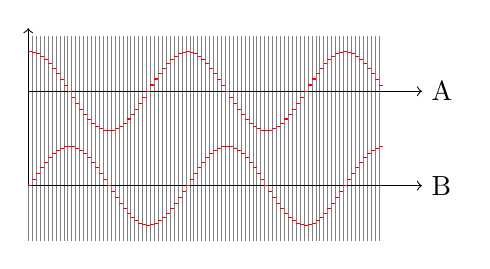
\begin{tikzpicture}
        % Hilfslinien
        \foreach \i in {0, 0.05, ..., 4.5}
        {
            \draw[ultra thin, gray] (\i, 1.9) -- (\i, -0.7);
        }
        % Achsen
    	\draw[->]	(0, 0) -- (0, 2);
    	\draw[->]	(0, 1.2) -- (5, 1.2) node[right]{A};
    	\draw[->]	(0, 0) -- (5, 0) node[right]{B};
        % Kurven
        \foreach \i in {0, 0.05, ..., 4.5}
        {
            \draw[red] (\i, {0.5*sin(180*\i)})          -- (\i+0.05, {0.5*sin(180*\i)});
            \draw[red] (\i, {0.5*sin(180*\i+(90))+1.2}) -- (\i+0.05, {0.5*sin(180*\i+(90))+1.2});
        }
    	\end{tikzpicture}
    	\caption{Mikroschritt}
    	\label{fig:mikroschritt}
    \end{figure}

    \noindent
    Wie bei anderen Motoren hat auch bei Schrittmotoren die Anzahl Polpaare 
    einen Einfluss auf dessen Drehzahl. Die Polpaare bilden eine Untersetzung 
    zwischen der elektrischen und der mechanischen Rotation. Die meisten 
    gängigen Schrittmotoren besitzen 50 Polpaare. Da eine elektrische 
    Umdrehung aus vier Schritten besteht ergeben sich bei 50 Polpaaren 200 
    Schritte für eine Umdrehung. Dies ergibt eine Schrittauflösung von 
    1.8\si{\degree} bei Vollschrittbetrieb. 

\ifSTANDALONE
    \subsection{Wicklungen} \label{sec:windings}
\fi
\ifEMBED
    \subsubsection{Wicklungen} \label{sec:windings}
\fi
    Ein Schrittmotor besitzt zwei getrennte Wicklungen. Diese sind 
    rechtwinklig zueinander angeordnet. Bei Motoren mit mehr als einem Polpaar 
    sind entsprechend mehr Wicklungen verbaut. Beim Aufbau der Wicklungen 
    wird zwischen unipolaren und bipolaren Wicklungen unterschieden. 
    %
    Die unipolare Wicklung besitzt einen Mittelabgriff. Dieser wird meistens 
    mit der Versorgungsspannung verbunden. Die beiden anderen Enden werden nun 
    mit einer Lowside Treiberstufe angesteuert. Dadurch kann der magnetische 
    Fluss mit einem geringen elektronischen Aufwand umgekehrt werden. Jedoch 
    ist immer nur eine Hälfte der Wicklung aktiv. Zudem ist die Herstellung 
    aufwendiger und somit auch teurer. 
    %
    Bei einer bipolaren Wicklung fehlt der mittlere Abgriff. Die Umkehrung des 
    magnetischen Flusses muss über die Umkehrung der angelegten Spannung 
    erfolgen. Deshalb muss für beide Wicklungen jeweils eine Brückenschaltung 
    verwendet werden. Da bei bipolaren Schrittmotoren immer die gesamte 
    Wicklung verwendet wird, kann damit ein grösseres Drehmoment erzeugt 
    werden als mit einem gleich grossen unipolaren Schrittmotor. 
    %
    Die Ansteuerung der beiden Wicklungsarten ist in \autoref{fig:uniVsbi} 
    ersichtlich. \cite{Doku:Stepper}
    \begin{figure}[h!]
       	\centering
       	\includegraphics[width=12cm]{\EtPath/Bilder/uniVsbi.jpg}
       	\caption[Bipolarer und unipolarer Betrieb]{bipolarer und unipolarer Betrieb \cite{Doku:Stepper}}
       	\label{fig:uniVsbi}
    \end{figure}
    
       
    
